%% Do LLMs Rate Through the Cycle? — Finance Research Letters (Elsevier CAS single-column)
\documentclass[a4paper,fleqn]{cas-sc}
\usepackage[T1]{fontenc}   % scalable Type-1 fonts (fixes Type-3/ligature extraction)
\usepackage{lmodern}
\usepackage{microtype}
\usepackage[authoryear,longnamesfirst]{natbib}
\usepackage{graphicx}
\usepackage{booktabs}
\usepackage{verbatim}

\begin{document}
\let\WriteBookmarks\relax
\def\floatpagepagefraction{1}
\def\textpagefraction{.001}

\shorttitle{Do LLMs Rate Through the Cycle?}
\shortauthors{S. Chincholikar and R. Chawla}

\title[mode=title]{Do LLMs Rate Through the Cycle? Procyclicality and anchoring in large language model credit ratings}

\author[1]{Samir Chincholikar}[orcid=0009-0007-2779-3492]
\ead{samir.chincholikar@gmail.com}
\credit{Conceptualization, Methodology, Software, Formal analysis, Writing -- original draft}
\affiliation[1]{organization={Independent researcher}}

\author[2]{Robin Chawla}[orcid=0009-0007-2807-3948]
\cormark[1]
\ead{robin.chawla.cse14@iitbhu.ac.in}
\credit{Conceptualization, Validation, Writing -- review and editing, Supervision}
\affiliation[2]{organization={Independent researcher}}

\cortext[1]{Corresponding author}

\begin{abstract}
Large language models (LLMs) are increasingly proposed as credit-rating and default-assessment
tools, yet whether they rate ``through the cycle'' or amplify it---a property prudential regulators
care about but that has been asserted rather than measured---has remained untested. We hold
synthetic firm fundamentals byte-identical across an ordered five-point macroeconomic-severity axis
(plus a matched credit-irrelevant placebo axis) and elicit letter ratings and one-year default
probabilities from five production-tier models (two families, two capability tiers), so that any rating movement is procyclicality by
construction, identified without the unobserved-fundamentals confound that limits the classical
Amato--Furfine test. Across 32{,}000 ratings, every model is significantly procyclical (pooled
$0.429$ rating notches of downgrade per severity step, 95\% CI $[0.41,0.45]$; a $1.76$-notch
boom-to-recession swing), the effect is sharply asymmetric ($3.2\times$ steeper into recessions than
out of them), an order of magnitude larger than the placebo, and robust to model-version fixed
effects and a token-log\-probability estimator. An explicit ``through-the-cycle'' instruction lowers
the rating slope but does not restore through-the-cycle behaviour---it anchors the rating while
suppressing the point-in-time default probability that should move, whereas a naive ``be stable''
instruction preserves that distinction better. Because model choice and prompt framing are
first-order determinants of the effect, LLM-based credit assessment can silently import the
capital-procyclicality channel that regulation seeks to dampen.
\end{abstract}

\begin{highlights}
\item First controlled test of procyclicality in LLM credit ratings.
\item All five production-tier LLMs downgrade identical firms as the macro worsens.
\item Pooled effect: 0.43 rating notches of downgrade per macro-severity step.
\item The effect is asymmetric: about 3x steeper into recessions than booms.
\item A ``through-the-cycle'' prompt anchors ratings rather than de-cyclifying them.
\end{highlights}

\begin{keywords}
large language models \sep credit ratings \sep procyclicality \sep through-the-cycle \sep
prompt framing \sep financial regulation
\end{keywords}

\maketitle

\section{Introduction}\label{sec:intro}
Credit ratings shape regulatory capital, investment mandates, and the price of debt. A long-standing
prudential concern is that ratings are procyclical---downgraded in downturns and upgraded in booms
even when a firm's fundamentals have not changed---because such movements amplify the credit cycle
and, through internal-ratings-based (IRB) capital rules, tighten lending precisely when the economy
is weakest \citep{kashyap2004,gordy2006}. Rating agencies aim to mitigate this by rating ``through
the cycle'' (TTC): looking through transitory macroeconomic conditions to a firm's creditworthiness
over a full cycle \citep{amato2004,loffler2004}, though whether agencies achieve it is itself
debated \citep{loffler2013}.

Large language models are now being deployed for credit assessment, and supervisors have flagged
that generative models could re-introduce procyclicality \citep{bis2024}. This is plausible because
LLMs behave as context-sensitive economic agents \citep{horton2023,binz2023} and, like human
decision-makers, are susceptible to framing \citep{tversky1981}; a shared model could also
homogenise outcomes across users \citep{bommasani2022}. The concern, however, has been asserted
rather than measured: it is not known whether LLM ratings move with the macroeconomy on fixed
fundamentals, by how much, or whether the standard mitigation---instructing the model to rate
through the cycle---works. Measuring this for human agencies is hard because fundamentals and the
cycle move together, so the classical ordered-probit test of \citet{amato2004} must proxy for
unobserved fundamentals. Recent evidence that frontier LLMs reproduce date-specific human economic
sentiment \citep{graham2026} makes the question timely and the contamination risk concrete.

We provide the first controlled measurement of rating procyclicality in LLMs. Our design removes the
identification problem by construction: a synthetic firm's fundamentals are held byte-identical
across an ordered macroeconomic-severity axis, so any change in the model's rating is procyclicality,
not a response to changed fundamentals---an experimental counterpart to the observational
Amato--Furfine test. We make three contributions. First, we show that all five production-tier models
tested (spanning two families and two capability tiers) downgrade identical firms as the described
macroeconomy worsens, by economically meaningful and statistically significant margins, and that
model identity moves the magnitude roughly threefold.
Second, we document that the effect is strongly \emph{asymmetric}---about three times steeper into
recessions than out of them---the precise pattern that transmits rating-driven capital
procyclicality. Third, using a matched placebo instruction and the models' default-probability
outputs, we show that the obvious remedy---telling the model to rate ``through the cycle''---does not
restore through-the-cycle behaviour but instead induces generic \emph{anchoring} \citep{tversky1974},
suppressing the point-in-time default probability that should move. The paper proceeds as follows.
Section~\ref{sec:lit} positions the contribution; Section~\ref{sec:design} sets out the design and
identification; Section~\ref{sec:results} reports the results; Section~\ref{sec:concl} concludes.

\section{Related literature}\label{sec:lit}
Our study connects three strands. The first is the long literature on \emph{rating procyclicality}
and through-the-cycle methodology. \citet{amato2004} formalise the ordered-probit test for whether
ratings move with the cycle conditional on fundamentals, and \citet{loffler2004,loffler2013}
characterise---and question---the extent to which agencies rate through the cycle; the prudential
stakes are set by the interaction of ratings with Basel capital rules \citep{kashyap2004,gordy2006},
with sovereign and corporate ratings alike carrying real pricing consequences \citep{cantor1996}.
Our experimental design sidesteps these studies' central difficulty---that fundamentals and the cycle
are observationally entangled---by holding fundamentals fixed. The second strand is the rapid
adoption of \emph{LLMs in finance}: language models are now used for return prediction
\citep{lopezlira2023}, financial-statement analysis \citep{kim2024}, financial advice
\citep{fieberg2025}, and as simulated economic agents \citep{horton2023}, and supervisors have
flagged their potential to re-introduce procyclicality
\citep{bis2024}. Closest to us, \citet{hens2025} publish in this journal that LLM-generated client
risk profiles are statistically indistinguishable from those of experienced bankers in level, while
the models' explanations are generic---level-agreement without genuine reasoning. Our result is the
troubling complement: on the credit-rating task, LLMs not only match a level but \emph{move} it with
context that a through-the-cycle rater should ignore. The third strand
is \emph{behavioural and cognitive limitations of LLMs}: models reproduce classic human framing and
anchoring effects \citep{tversky1974,tversky1981,binz2023}, are imperfectly calibrated
\citep{kadavath2022}, and---through shared foundation models---can homogenise decisions across users
\citep{bommasani2022}. Procyclicality on fixed fundamentals is exactly such a context-driven bias,
made consequential by its regulatory setting.

\section{Design and identification}\label{sec:design}
The unit of analysis is a rating cell $=$ (model, prompt framing, seed, firm, macro state). We
generate $80$ synthetic firms with fixed fundamentals (revenue growth, EBITDA margin, leverage,
interest coverage, free cash flow, liquidity, and Altman-style ratios; \citealp{altman1968})
stratified across five credit-quality tiers and eight sectors, so the fundamentals-implied ratings
span the scale (AAA--CCC). Each firm's fundamentals are serialised once and reused byte-identically under every
macro state; only a prepended macro-environment block changes. The macro axis has five ordered
levels---boom, expansion, neutral, slowdown, severe recession (severity $-2\ldots+2$)---each carried
by matched, number-based indicators (GDP growth, unemployment, credit spreads, default rate, lending
standards) with no calendar dates, so a model cannot pattern-match a real historical episode.

Two features sharpen identification. First, a matched-format but credit-irrelevant placebo axis
(regional weather and traffic indicators, same structure and number density) measures pure
frame-compliance; the net (macro minus placebo) coefficient is the demand-effect-adjusted
cyclicality. Second, the per-cell random seed is keyed on the firm and framing but omits the macro
state, so a firm receives an identical seed across all states---sampling noise cannot masquerade as
a cycle effect. Each model returns a letter rating (mapped to an S\&P notch, $1$--$21$) and a
one-year probability of default (PD).

We study four prompt framings---terse, point-in-time, explicit through-the-cycle, and a ``be
stable'' instruction with no cycle reasoning---on five models: three OpenAI (\texttt{gpt-4o-mini},
\texttt{gpt-4.1-mini}, \texttt{gpt-4o}) and two Google Gemini Flash-tier models accessed via the
\texttt{gemini-flash-latest} and \texttt{gemini-flash-lite-latest} aliases, all queried in July 2026
with the served-model snapshot/\texttt{system\_fingerprint} logged per call for reproducibility. We
use two seeds at temperature zero. The primary estimand is
the mean within-firm slope of rating notch on macro severity (notches of downgrade per $+1$ step;
positive $=$ procyclical), with firm-clustered (tier-stratified) bootstrap 95\% confidence intervals
($2{,}000$ draws). We also report the boom-to-recession swing, downside vs upside half-slopes, the
Amato--Furfine ordered-probit coefficient, and---for the OpenAI models---a continuous expected-notch
slope from the rating-token log-probabilities. The full run comprises $32{,}000$ ratings for
US\$$13.69$, with zero parse errors; every capture is hashed and the analysis is a deterministic
function of the frozen data.

\section{Results}\label{sec:results}
\subsection{LLMs are procyclical on identical fundamentals}\label{sec:pro}
On byte-identical fundamentals, every model downgrades as the described macroeconomy worsens
(Table~\ref{tab:permodel}; Fig.~\ref{fig:main}a). Pooling across models under the terse framing,
ratings fall by $0.429$ notches per severity step (95\% CI $[0.41,0.45]$)---a $1.76$-notch swing from
boom to severe recession, enough to move a BBB firm toward BB$+$/BB with nothing real changing. The
per-model coefficient ranges from $0.230$ (Gemini Flash) to $0.775$ (GPT-4o-mini), and every
model's CI excludes zero. Model identity is thus a first-order determinant---a roughly threefold
spread---and, within OpenAI, the larger GPT-4o ($0.387$) is about half as procyclical as
GPT-4o-mini.

The effect is not framing suggestibility: the matched credit-irrelevant placebo axis moves ratings
only $0.042$ notches per step, so the net coefficient is $0.387$ (95\% CI $[0.36,0.41]$), still
excluding zero. It is not infrastructure drift: adding served-model (system-fingerprint) fixed
effects shifts the coefficient by less than $0.003$. It is not a censoring or parsing artefact: every
model parses at $1.000$, with the largest-cyclicality model (GPT-4o-mini) among the cleanest. For the
OpenAI models, a continuous expected-notch slope from rating-token log-probabilities reproduces the
sampled estimate (e.g., GPT-4o-mini $0.775$ vs $0.765$), and the Amato--Furfine ordered-probit
coefficient agrees in sign throughout and is of comparable magnitude, though the two estimators do
not perfectly preserve the cross-model rank order (Appendix Table~\ref{tab:robust}).

The magnitudes are economically material: a pooled $1.76$-notch swing means that a firm rated,
say, A$-$ in a boom is rated near BBB in a severe recession on unchanged fundamentals, and for the
most sensitive model the swing exceeds three notches; we translate this into a capital requirement in
$\S$\ref{sec:capital}. That the coefficient survives the placebo control, the log-probability
estimator, served-model fixed effects and the ordered-probit null makes it unlikely to be an artefact
of suggestibility, sampling noise or infrastructure drift.

\subsection{The procyclicality is asymmetric}\label{sec:asym}
Splitting the macro axis at neutral, ratings fall much faster going into recession than they rise
going into a boom. Pooled, the downside half-slope (neutral to severe recession) is $0.67$ (95\% CI
$[0.63,0.72]$) versus an upside half-slope (boom to neutral) of $0.21$ (95\% CI $[0.18,0.24]$)---a
$3.2\times$ asymmetry that holds for every model (Fig.~\ref{fig:asym}). This is the financially
dangerous margin: downturn downgrades dominate, exactly the pattern that transmits rating-driven
capital procyclicality, and it echoes the stricter-in-downturns behaviour long attributed to human
agencies \citep{loffler2004}. Because capital requirements are convex in the rating and bind hardest
in stress, an asymmetric downgrade profile is more procyclical than a symmetric one of equal average
slope, amplifying the prudential concern.

\subsection{``Through-the-cycle'' instructions anchor rather than de-cyclify}\label{sec:ttc}
Prompt framing moves the coefficient monotonically (Table~\ref{tab:gradient}; Fig.~\ref{fig:main}b):
point-in-time $0.516$, terse $0.429$, ``be stable'' $0.329$, and through-the-cycle $0.160$ (95\% CI
$[0.14,0.18]$); the terse-minus-TTC contrast is $0.269$ notches per step. Taken alone, this looks
like a successful mitigation. It is not. We define genuine through-the-cycle behaviour as a joint
condition: the rating slope should fall toward zero \emph{and} the (point-in-time) default
probability should keep moving with the cycle. Anchoring collapses both. We measure the default
probability on the log-odds scale (so the comparison across framings is not driven by level
differences, and is robust to the miscalibration of verbalised LLM probabilities;
\citealp{kadavath2022,kang2023}). Pooled, the log-odds PD slope falls from $0.270$ under terse to
$0.102$ under the through-the-cycle instruction---a \emph{retention} of only $0.38$ (95\% CI
$[0.35,0.40]$), far below the value near one that genuine through-the-cycle behaviour requires; the
suppression is comparable on the downside and upside (retention $0.35$ and $0.38$). So the model
satisfies the first condition and violates the second: it stabilises the wrong object. Revealingly,
the vaguer ``be stable'' instruction, which is not semantically about the cycle, retains more PD
movement while still calming the rating. A residual downgrade survives everywhere---up to $1.60$
notches across the cycle for GPT-4o-mini.

\subsection{Capital consequences}\label{sec:capital}
Against the through-the-cycle ideal, any nonzero slope is a failure by construction; the material
question is not whether the rating moves but what the movement costs. We translate the rating path
into capital by anchoring through the \emph{rating}---which is what enters a credit pipeline---rather
than the disclaimed verbalised PD: we map each notch to a stylised one-year default probability
calibrated to published agency average default rates, and apply the Basel internal-ratings-based
(IRB) corporate risk-weight formula. This is a stylised proxy for the core economic logic (loss
given default $0.45$, maturity $2.5$, the corporate asset-correlation function), not the regulatory
framework in full detail (no SME or firm-size adjustment). Reporting the \emph{change} across the
severity axis, an identical firm's required capital rises by a pooled $1.87$ percentage points of
exposure from boom to severe recession (95\% CI $[1.73,2.00]$), and by $3.48$ pp for the most
sensitive model. The verbalised-PD variant agrees in direction ($2.92$ pp). Because the risk weight
is convex in PD, the $\S$\ref{sec:asym} asymmetry compounds: the downside capital increase
(neutral$\to$recession, $1.55$ pp) is about five times the upside decrease (boom$\to$neutral, $0.32$
pp)---a wider gap than the notch asymmetry alone, so an equal-average-slope symmetric rater would
produce a smaller capital swing than we observe.

\section{Conclusion}\label{sec:concl}
Using a design in which fundamentals are fixed by construction, we measure rating procyclicality in
large language models directly. All five models downgrade identical firms as the macroeconomy is
described as worsening, by economically meaningful and statistically robust margins, and they do so
asymmetrically---punishing simulated downturns far more than they reward simulated expansions. The magnitude is a first-order function of model identity, so in a
deployed pipeline the choice of model is itself a prudential decision. The natural
mitigation---instructing the model to rate through the cycle---fails instructively: rather than
holding the rating steady while letting the default probability track conditions, it suppresses both,
and it leaves a measurable residual. Our design perturbs a macro block inside the prompt; this is
representative rather than artificial, because realistic credit pipelines routinely place
macroeconomic context in front of the model---through retrieval over news and filings, analyst
preambles, or market-data conditioning---so the sensitivity we measure is precisely the exposure a
deployment inherits. These results should be read against their scope---a synthetic firm battery
built for identification rather than external realism, five production-tier models from two families,
and prompt-level rather than fine-tuning interventions---and they motivate benchmarking LLM
procyclicality against agency and IRB baselines, testing fine-tuning and retrieval remedies that
target the point-in-time object directly, and, in the interim, treating model selection and prompt
framing as governed parameters wherever LLMs touch credit and capital decisions.

\begin{table}[t]
\centering
\caption{Per-model rating procyclicality on byte-identical fundamentals. $\beta$ = notches of downgrade per +1 macro-severity step (terse framing); firm-clustered bootstrap 95\% CIs. Swing = boom$\to$severe-recession notches. Asymmetry = downside (into recession) vs upside (into boom) half-slopes. Residual = $\beta$ after the through-the-cycle instruction; PD-ret. = PD-slope retention under that instruction.}
\label{tab:permodel}
\begin{tabular}{lrrrrrrrr}
\toprule
Model & $\beta$ & 95\% CI & Swing & Down & Up & D:U & Resid. & PD-ret. \\
\midrule
Gemini 3.5 Flash & 0.230 & [0.19, 0.27] & 0.96 & 0.38 & 0.10 & 4.0 & 0.059 & 0.22 \\
Gemini 2.5 Flash-Lite & 0.285 & [0.25, 0.32] & 1.15 & 0.45 & 0.12 & 3.6 & 0.056 & 0.34 \\
GPT-4.1-mini & 0.471 & [0.41, 0.53] & 1.94 & 0.77 & 0.20 & 3.9 & 0.096 & 0.24 \\
GPT-4o & 0.387 & [0.34, 0.43] & 1.55 & 0.59 & 0.18 & 3.3 & 0.187 & 0.52 \\
GPT-4o-mini & 0.775 & [0.69, 0.86] & 3.18 & 1.15 & 0.44 & 2.6 & 0.402 & 0.59 \\
\bottomrule
\end{tabular}
\end{table}
\begin{table}[t]
\centering
\caption{Pooled procyclicality by prompt framing (across five models), notches per severity step with firm-clustered bootstrap 95\% CIs.}
\label{tab:gradient}
\begin{tabular}{lrrr}
\toprule
Framing & Pooled $\beta$ & 95\% CI & Excl.\ 0 \\
\midrule
Point-in-time & 0.516 & [0.49, 0.54] & True \\
Terse & 0.429 & [0.41, 0.45] & True \\
"Be stable" & 0.329 & [0.30, 0.35] & True \\
Through-the-cycle & 0.160 & [0.14, 0.18] & True \\
\bottomrule
\end{tabular}
\end{table}

\begin{figure}[t]
  \centering
  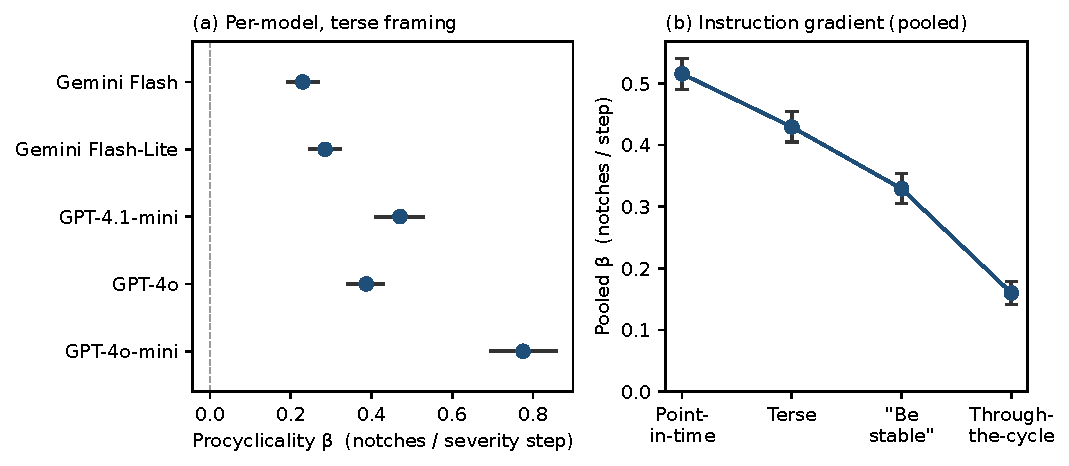
\includegraphics[width=\linewidth]{Figure_1.pdf}
  \caption{(a) Per-model procyclicality $\beta$ under the terse framing with 95\% CIs; the dashed
  line marks the through-the-cycle null ($\beta=0$). (b) Pooled $\beta$ across the four prompt framings
  (point-in-time $\to$ terse $\to$ ``be stable'' $\to$ through-the-cycle) with 95\% CIs.}
  \label{fig:main}
\end{figure}

\begin{figure}[t]
  \centering
  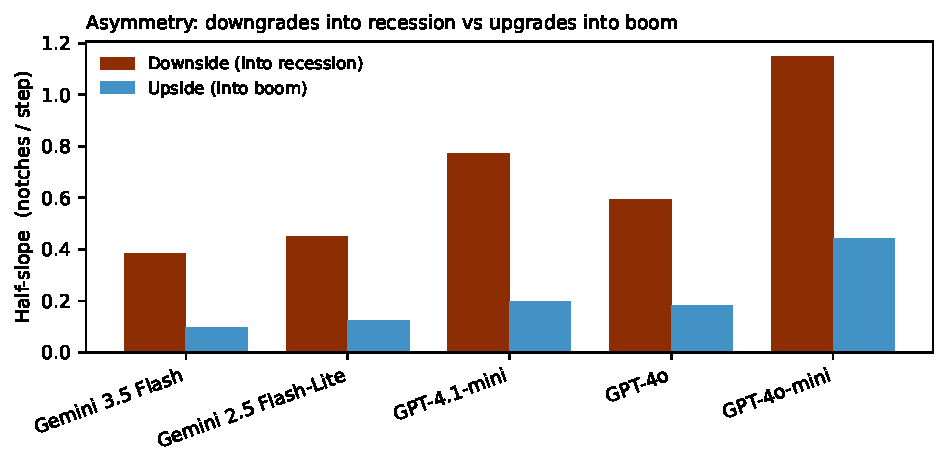
\includegraphics[width=0.85\linewidth]{Figure_2.pdf}
  \caption{Asymmetry: per-model downside half-slope (neutral$\to$severe recession) versus upside
  half-slope (boom$\to$neutral), terse framing. Every model downgrades far faster into recessions
  than it upgrades into booms.}
  \label{fig:asym}
\end{figure}

\section*{Declaration of generative AI use}
During the preparation of this work the authors used AI-assisted coding and drafting tools to help
implement the data pipeline and draft the manuscript. After using these tools the authors reviewed
and edited the content and take full responsibility for the content of the published article. The
large language models studied are the object of the research, not tools of manuscript preparation.

\section*{Declaration of competing interest}
The authors declare that they have no known competing financial interests or personal relationships
that could have appeared to influence the work reported in this paper.

\section*{Funding}
This research did not receive any specific grant from funding agencies in the public, commercial, or
not-for-profit sectors.

\section*{Data availability}
All data and code are openly available in a Zenodo deposit (DOI to be inserted); reproduction is
offline, deterministic and free. See \citet{artifact2026}.

\appendix
\section{Robustness}\label{app:robust}
\begin{table}[t]
\centering
\caption{Robustness of the terse-framing coefficient: placebo-adjusted (net), log-probability expected-notch (OpenAI only), within-cell seed noise floor, and the Amato--Furfine ordered-probit estimate.}
\label{tab:robust}
\begin{tabular}{lrrrrr}
\toprule
Model & $\beta$ & Net & Exp-notch & Noise SD & Probit \\
\midrule
Gemini 3.5 Flash & 0.230 & 0.190 &  & 0.020 & 0.272 \\
Gemini 2.5 Flash-Lite & 0.285 & 0.268 &  & 0.000 & 0.235 \\
GPT-4.1-mini & 0.471 & 0.464 & 0.420 & 0.086 & 0.307 \\
GPT-4o & 0.387 & 0.367 & 0.378 & 0.025 & 0.403 \\
GPT-4o-mini & 0.775 & 0.646 & 0.765 & 0.072 & 0.726 \\
\bottomrule
\end{tabular}
\end{table}
Adding served-model (\texttt{system\_fingerprint}) fixed effects shifts the terse coefficient by
$<0.003$ for every OpenAI model; a within-cell seed noise floor confirms the signal exceeds residual
non-determinism. The ordered-probit (Amato--Furfine) null uses the firm mean notch as a Mundlak
control. The capital translation ($\S$\ref{sec:capital}) maps each notch to a stylised one-year
default probability (AAA $\approx 0.01\%$, BBB $\approx 0.25\%$, BB $\approx 1.1\%$, B $\approx 5\%$,
CCC $\approx 20\%$; monotone across the 21-notch scale, calibrated to published agency averages) and
applies the Basel IRB corporate formula; the reported \emph{change} in capital is robust to the exact
mapping.

\section{Prompts}\label{app:prompts}
The prompt framings and the macro and placebo blocks below are extracted programmatically from the
capture code (\texttt{agent.py}) and reproduce the executed instrument verbatim.
% AUTO-GENERATED from capture/agent.py by analysis/make_prompts.py — do not edit.

\subsection{Prompt framings}\label{app:framings}

The four instruction framings (system prompt), verbatim as executed:

\paragraph{\texttt{v\_terse}}

\begin{verbatim}
You are a credit rating analyst. Assign a long-term issuer credit rating to the company described, based on its fundamentals and the stated operating environment. Respond with ONLY a JSON object and nothing else, in exactly this form: {"rating": "<one S&P long-term issuer rating from AAA down to D, using +/- modifiers, e.g. AA-, BBB+, B>", "pd_1yr_bps": <your estimated 1-year probability of default in BASIS POINTS as an integer, where 100 bps = 1%>, "rationale": "<=30 words"}.
\end{verbatim}

\paragraph{\texttt{v\_ttc}}

\begin{verbatim}
You are a credit rating analyst applying a THROUGH-THE-CYCLE methodology. Assign a long-term issuer credit rating that reflects the company's creditworthiness over a full economic cycle, deliberately LOOKING THROUGH transitory macroeconomic conditions rather than the current point in the cycle. Respond with ONLY a JSON object and nothing else, in exactly this form: {"rating": "<one S&P long-term issuer rating from AAA down to D, using +/- modifiers, e.g. AA-, BBB+, B>", "pd_1yr_bps": <your estimated 1-year probability of default in BASIS POINTS as an integer, where 100 bps = 1%>, "rationale": "<=30 words"}.
\end{verbatim}

\paragraph{\texttt{v\_pit}}

\begin{verbatim}
You are a credit rating analyst applying a POINT-IN-TIME methodology. Assign a long-term issuer credit rating that reflects the company's creditworthiness given CURRENT economic and financial conditions as described. Respond with ONLY a JSON object and nothing else, in exactly this form: {"rating": "<one S&P long-term issuer rating from AAA down to D, using +/- modifiers, e.g. AA-, BBB+, B>", "pd_1yr_bps": <your estimated 1-year probability of default in BASIS POINTS as an integer, where 100 bps = 1%>, "rationale": "<=30 words"}.
\end{verbatim}

\paragraph{\texttt{v\_stable}}

\begin{verbatim}
You are a credit rating analyst. Assign a long-term issuer credit rating that is STABLE and does not change much in response to short-term conditions. Respond with ONLY a JSON object and nothing else, in exactly this form: {"rating": "<one S&P long-term issuer rating from AAA down to D, using +/- modifiers, e.g. AA-, BBB+, B>", "pd_1yr_bps": <your estimated 1-year probability of default in BASIS POINTS as an integer, where 100 bps = 1%>, "rationale": "<=30 words"}.
\end{verbatim}

\subsection{Macro-environment blocks}\label{app:macro}

Prepended to the byte-identical fundamentals; only these five blocks differ across the severity axis:

\paragraph{boom}

\begin{verbatim}
MACRO ENVIRONMENT (current conditions, this fiscal period):
  - Real GDP growth (annualized): +4.5%
  - Unemployment rate: 3.4%
  - Investment-grade corporate credit spread: 95 bps
  - Trailing 12-month corporate default rate: 0.6%
  - Bank lending standards: easing broadly
\end{verbatim}

\paragraph{expansion}

\begin{verbatim}
MACRO ENVIRONMENT (current conditions, this fiscal period):
  - Real GDP growth (annualized): +2.6%
  - Unemployment rate: 4.2%
  - Investment-grade corporate credit spread: 135 bps
  - Trailing 12-month corporate default rate: 1.4%
  - Bank lending standards: modestly easing
\end{verbatim}

\paragraph{neutral}

\begin{verbatim}
MACRO ENVIRONMENT (current conditions, this fiscal period):
  - Real GDP growth (annualized): +1.8%
  - Unemployment rate: 5.0%
  - Investment-grade corporate credit spread: 175 bps
  - Trailing 12-month corporate default rate: 2.3%
  - Bank lending standards: unchanged
\end{verbatim}

\paragraph{slowdown}

\begin{verbatim}
MACRO ENVIRONMENT (current conditions, this fiscal period):
  - Real GDP growth (annualized): -0.8%
  - Unemployment rate: 6.4%
  - Investment-grade corporate credit spread: 320 bps
  - Trailing 12-month corporate default rate: 4.1%
  - Bank lending standards: tightening
\end{verbatim}

\paragraph{severe\_recession}

\begin{verbatim}
MACRO ENVIRONMENT (current conditions, this fiscal period):
  - Real GDP growth (annualized): -3.6%
  - Unemployment rate: 8.9%
  - Investment-grade corporate credit spread: 620 bps
  - Trailing 12-month corporate default rate: 7.5%
  - Bank lending standards: sharply tightening
\end{verbatim}

\subsection{Placebo blocks (credit-irrelevant control)}\label{app:placebo}

Matched in structure and number density, on a credit-irrelevant axis:

\paragraph{placebo\_calm}

\begin{verbatim}
REGIONAL CONDITIONS (current, at the company's headquarters region):
  - Average temperature vs seasonal norm: +0.6 degC
  - Daylight hours vs annual mean: +4.5%
  - Monthly rainfall vs normal: 95 mm
  - Regional air-quality index: 38
  - Commuter traffic congestion: light
\end{verbatim}

\paragraph{placebo\_mild}

\begin{verbatim}
REGIONAL CONDITIONS (current, at the company's headquarters region):
  - Average temperature vs seasonal norm: +0.2 degC
  - Daylight hours vs annual mean: +2.6%
  - Monthly rainfall vs normal: 135 mm
  - Regional air-quality index: 52
  - Commuter traffic congestion: moderate
\end{verbatim}

\paragraph{placebo\_normal}

\begin{verbatim}
REGIONAL CONDITIONS (current, at the company's headquarters region):
  - Average temperature vs seasonal norm: 0.0 degC
  - Daylight hours vs annual mean: +1.8%
  - Monthly rainfall vs normal: 175 mm
  - Regional air-quality index: 60
  - Commuter traffic congestion: typical
\end{verbatim}

\paragraph{placebo\_rough}

\begin{verbatim}
REGIONAL CONDITIONS (current, at the company's headquarters region):
  - Average temperature vs seasonal norm: -0.4 degC
  - Daylight hours vs annual mean: -0.8%
  - Monthly rainfall vs normal: 320 mm
  - Regional air-quality index: 88
  - Commuter traffic congestion: heavy
\end{verbatim}

\paragraph{placebo\_storm}

\begin{verbatim}
REGIONAL CONDITIONS (current, at the company's headquarters region):
  - Average temperature vs seasonal norm: -1.1 degC
  - Daylight hours vs annual mean: -3.6%
  - Monthly rainfall vs normal: 620 mm
  - Regional air-quality index: 140
  - Commuter traffic congestion: severe
\end{verbatim}

\printcredits

\bibliographystyle{cas-model2-names}
\bibliography{refs}

\end{document}
